\documentclass[aps,prb,twocolumn,superscriptaddress,floatfix,longbibliography,10pt]{revtex4-2}

\usepackage[utf8]{inputenc}
\usepackage[spanish]{babel}
\usepackage{graphicx}
\usepackage{amsmath}
\usepackage{subcaption}
\usepackage{wrapfig} 
\usepackage[export]{adjustbox}

\usepackage{amsmath,amssymb} % math symbols
\usepackage{bm} % bold math font
\usepackage{graphicx} % for figures
\usepackage{comment} % allows block comments
\usepackage{textcomp} % This package is just to give the text quote '
%\usepackage{ulem} % allows strikeout text, e.g. \sout{text}

\usepackage[spanish]{babel}
% By dafault, spanish changes to a comma as decimal separator; to change to a dot, you can use \decimalpoint:
\decimalpoint

\usepackage{enumitem}
\setlist{noitemsep,leftmargin=*,topsep=0pt,parsep=0pt}

\usepackage{xcolor} % \textcolor{red}{text} will be red for notes
\definecolor{lightgray}{gray}{0.6}
\definecolor{medgray}{gray}{0.4}

%Para las tablas
\usepackage{multirow}

\usepackage{hyperref}
\hypersetup{
colorlinks=true,
urlcolor= blue,
citecolor=blue,
linkcolor= blue,
bookmarks=true,
bookmarksopen=false,
}

% Code to add paragraph numbers and titles
\newif\ifptitle
\newif\ifpnumber
\newcounter{para}
\newcommand\ptitle[1]{\par\refstepcounter{para}
{\ifpnumber{\noindent\textcolor{lightgray}{\textbf{\thepara}}\indent}\fi}
{\ifptitle{\textbf{[{#1}]}}\fi}}
\ptitletrue  % comment this line to hide paragraph titles
\pnumbertrue  % comment this line to hide paragraph numbers

% minimum font size for figures
\newcommand{\minfont}{6}

% Uncomment this line if you prefer your vectors to appear as bold letters.
% By default they will appear with arrows over them.
% \renewcommand{\vec}[1]{\bm{#1}}

%Cambiar Cuadros por Tablas y lista de...
%\renewcommand{\listtablename}{Índice de tablas}
\renewcommand{\tablename}{Tabla}
\renewcommand{\date}{Fecha}

%Para importar imágenes desde una carpeta:
\graphicspath{ {C:/Users/lupam/OneDrive/Escritorio/GitHub/Metodos_Num_Fluidos_I/Guias/Informe_final/Informe/Figures} {C:/Users/lupam/OneDrive/Escritorio/GitHub/Metodos_Num_Fluidos_I/Guias/Informe_final/Programa/graficos}}

\usepackage[bottom]{footmisc} %para que las notas al pie aparezcan en la misma página

\begin{comment}

%Comandos de interés:

* Para ordenar el documento:
\section{Introducción}
\section{\label{sec:Formatting}Formatting} %label para luego hacer referencia a esa sección

\ptitle{Start writing while you experiment} %pone nombre y título al documento dependiendo de si en el header están los comandos \ptitletrue y \pnumbertrue

* Ecuaciones:
\begin{equation}
a^2+b^2=c^2 \,.
\label{eqn:Pythagoras}
\end{equation}

* Conjunto de ecuaciones:
\begin{eqnarray}
\label{eqn:diagonal}
\nonumber d & = & \sqrt{a^2 + b^2 + c^2} \\
& = & \sqrt{3^2+4^2+12^2} = 13
\end{eqnarray}

* Para hacer items / enumerar:
\begin{enumerate}
  \item
\end{enumerate}

\begin{itemize}
  \item
\end{itemize}

* Figuras:
\begin{figure}[h]
    \includegraphics[clip=true,width=\columnwidth]{pixel-compare}
    \caption{}
     \label{fig:pixels}
\end{figure}

* Conjunto de figuras:
\begin{figure}
     \centering
     \begin{subfigure}[b]{0.3\textwidth}
         \centering
         \includegraphics[width=\textwidth]{graph1}
         \caption{$y=x$}
         \label{fig:y equals x}
     \end{subfigure}
     \hfill
     \begin{subfigure}[b]{0.3\textwidth}
         \centering
         \includegraphics[width=\textwidth]{graph2}
         \caption{$y=3sinx$}
         \label{fig:three sin x}
     \end{subfigure}
     \hfill
     \begin{subfigure}[b]{0.3\textwidth}
         \centering
         \includegraphics[width=\textwidth]{graph3}
         \caption{$y=5/x$}
         \label{fig:five over x}
     \end{subfigure}
        \caption{Three simple graphs}
        \label{fig:three graphs}
\end{figure}


* Para hacer referencias a fórmulas, tablas, secciones, ... dentro del documento:
\ref{tab:spacing}

* Para citar
Elementos de .bib
\cite{WhitesidesAdvMat2004}
url
\url{http://www.mendeley.com/}\\

* Agradecimientos:
\begin{acknowledgments}
We acknowledge advice from Jessie Zhang and Harry Pirie to produce Fig.\ \ref{fig:pixels}.
\end{acknowledgments}

* Apéndice:
\appendix
\section{\label{app:Mendeley}Mendeley}

* Bibliografía:
\bibliography{Hoffman-example-paper}

\end{comment}



\begin{document}

% Allows to rewrite the same title in the supplement
\newcommand{\mytitle}{\textcolor{red}{Título??}}

\title{\mytitle}

\author{Pablo Chehade \\
    \small \textit{pablo.chehade@ib.edu.ar} \\
    \small \textit{Métodos Numéricos en Fluidos I, Instituto Balseiro, CNEA-UNCuyo, Bariloche, Argentina, 2022} \\}


\begin{abstract}

\begin{itemize}
  \item Se estudiaron métodos numéricos espaciales y de evolución temporal para resolver el problema de la cavidad cuadrada hidrodinámica bidimensional.
  \item Se tiene en cuenta la ecuación de momentos y la de conservación de masa. Este tiene un término advectivo, uno difusivo.
  \item Se resolvió mediante el método de volumenes finitos y algoritmo simpler calculando presión y velocidades con grilla desplazada.
  \item En primer lugar, se estudió la dependencia de la solución en el estado estacionario con respecto al paso temporal.
  \item Se planteó un algoritmo para minimizar el costo computacional para encontrar el estado estacionario con un error menor al 5 \%
  \item En segundo lugar, se estudió el impacto en el estacionario del esquema espacial en el término advectivo empleando distintos números de Reynolds. En particular, se utilizaron diferencias centradas de orden 2, Up-wind de orden uno y el esquema QUICK de orden \textcolor{red}{?}
  \item Además, se estudió el orden de convergencia espacial de Up-wind de primer orden en referencia al mejor esquema advectivo
  \item Se evaluó el efecto de los pasos internos del algoritmo simpler
  \item Se estudió el efecto del método de evolución temporal, evaluando el estado transitorio de la solución mediante los métodos Euler Implícito y Crank-Nicholson
\end{itemize}


\end{abstract}

\maketitle

\textcolor{red}{Dudas:}
\begin{itemize}
  \item A mayor Re, mayor dt?
  \item $t_hat = tU_0/L$
\end{itemize}

\section{Introducción}

\ptitle{¿Por qué es importante resolver problemas de fluidos numéricamente? Rtas en la primera clase}

Gran parte de los problemas de mecánica de fluidos no son resolubles analíticamente. Algunos de ellos pueden ser estudiados experimentalmente, con el costo operativo y las dificultades para realizar las mediciones que esto conlleva \textcolor{red}{ref clase 1}. Una alternativa más rápida y de menor costo es resolverlos numéricamente. Si bien esto trae aparejado algunas dificultades, como los errores de aproximación numérica y el costo computacional, en los últimos años la resolución numérica de ecuaciones es aceptada y está ganando preponderancia.

\ptitle{Explicar el problema de la cavidad cuadrada hidrodinámica bidimensional}
Un problema muy estudiado desde el punto de vista numérico en mecánica de fluidos es el de la cavidad cuadrada hidrodinámica bidimensional, también conocido como Shear-drien cavity flow. En la figura \ref{fig:esquema_cavidad_cuadrada} se muestra un esquema del mismo. Consiste en una cavidad cuadrada bidimensional de lado $L$ que contiene un fluido incompresible de viscocidad $\nu$. Las condiciones de borde son de no deslizamiento en todas las paredes excepto en la horizontal superior. Sea $\vec{V}(x,y,t) = (u(x,y,t), v(x,y,t))$ la velocidad en el punto $(x,y)$ a tiempo $t$, las condiciones anteriores se traducen en $\vec{V}(x,0) = \vec{V}(0,y) = \vec{V}(L,y) = (0,0)$ y $\vec{V}(x,L) = (U_0(t),0)$.
\end{itemize}

\begin{figure}[h]
  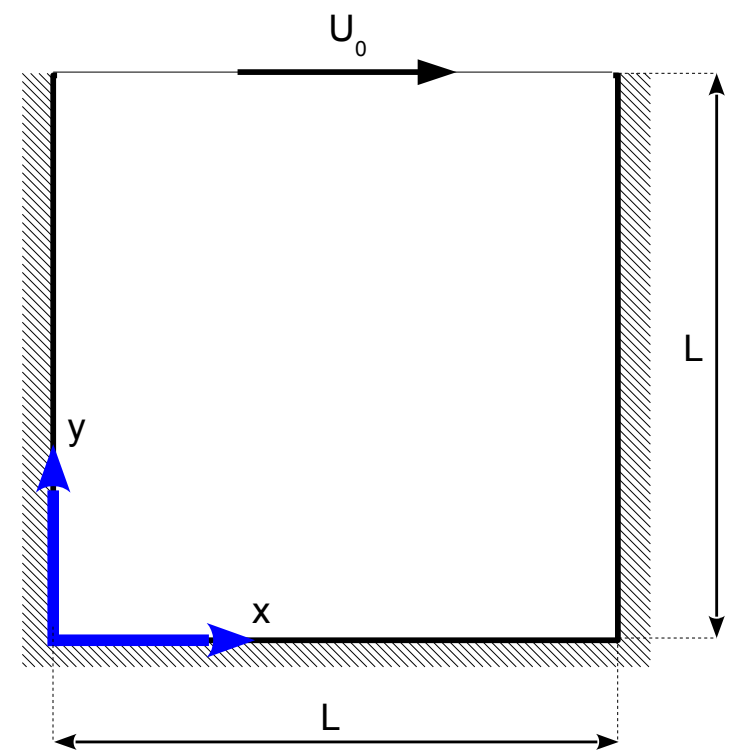
\includegraphics[clip=true,width=0.7\columnwidth]{esquema_cavidad_cuadrada.png}
  \caption{Esquema del problema de la cavidad cuadrada hidrodinámica bidimensional. Consiste en una cavidad cuadrada bidimensional de lado $L$ que contiene un fluido incompresible de viscocidad $\nu$. Las condiciones de borde son de no deslizamiento en todas las paredes excepto en la horizontal superior, con velocidad $U_0$. Esta figura fue extraída de \cite{Notas_materia}.}
   \label{fig:esquema_cavidad_cuadrada}
\end{figure}


\ptitle{Explicación de las ecuaciones involucradas}

El objetivo es determinar la presión $p(x,y,t)$ y las velocidades $u(x,y,t)$ y $v(x,y,t)$ para todo punto $(x,y)$ y tiempo $t$. Para esto se cuenta con tres ecuaciones diferenciales. En primer lugar, la ecuación de conservación de momento en las direcciones vertical y horizontal. Adimensionalmente, estas son
\begin{equation}
  \frac{\partial u}{\partial t} + \frac{\partial (u u)}{\partial x} + \frac{\partial (u v)}{\partial y} = - \frac{\partial p}{\partial x} + \frac{1}{Re} \left ( \frac{\partial^2 u}{\partial x^2} + \frac{\partial^2 u}{\partial y^2} \right ),
  \label{eq:momento_x}
\end{equation}
\begin{equation}
  \frac{\partial v}{\partial t} + \frac{\partial (u v)}{\partial x} + \frac{\partial (v v)}{\partial y} = - \frac{\partial p}{\partial y} + \frac{1}{Re} \left ( \frac{\partial^2 v}{\partial x^2} + \frac{\partial^2 v}{\partial y^2} \right ),
  \label{eq:momento_y}
\end{equation}
donde $Re = U_0L/\nu$ es el número de Reynolds. En ambas ecuaciones, el primer término del lado izquierdo resume la dependencia temporal del problema, los términos siguientes corresponden al efecto advectivo, el primer término del lado derecho resume la dependencia con la presión y los siguientes, el efecto difusivo. En segundo lugar se cuenta con la ecuación de conservación de masa. Para un fluido incompresible esta es
\begin{equation}
  \bigtriangledown \bullet \vec{V} = \frac{\partial u}{\partial x} + \frac{\partial v}{\partial y} = 0.
  \label{eq:cons_masa}
\end{equation}


En base a esta ecuación se suele decir que el campo de velocidades tiene divergencia libre.

\ptitle{Resumen}

Empleando las tres ecuaciones diferenciales en derivadas parciales anteriores, es posible calcular la presión y las velocidades. Es notable que las soluciones dependerán del valor del número de Reynolds, el cual depende de la velocidad en la cara superior, la longitud de la cavidad y la viscocidad del líquido.

\section{Métodos Numéricos}

\ptitle{Resumen}
Para resolver el sistema de ecuaciones diferenciales es necesario discretizar el dominio y plantear esquemas numéricos para las ecuaciones diferenciales. En cuanto al primero, es necesario diferenciar entre dominio espacial y temporal. En cuanto al segundo, se emplearon volúmenes finitos con el objetivo de asegurar la conservación de masa \textcolor{red}{?} y se estudió el efecto de distintos métodos espaciales y temporales.

\subsection{Discretización del dominio}

\ptitle{Discretización espacial}
El dominio espacial se discretiza mediante una grilla uniforme con igual espaciamiento $\Delta$ en ambas direcciones. El número de volúmenes por dirección espacial es $n$ tal que $\Delta = 1/n$. En total se cuentan con $n^2$ volúmenes, cada uno numerado con los índices $i$ y $j$ para las direcciones horizontales y verticales, respecticamente.

\ptitle{Grilla desplazada}
Se emplearon grillas desplazadas para las velocidades y la presión. Estas se muestran esquemáticamente en la figura \ref{fig:grillas_desplazadas}. De este modo, $P_{ij}$ es la presión en el volumen de tamaño $\Delta \times \Delta$ ubicado en $x = i \Delta$ e $y = j \Delta$. Mientras que $U_{ij}$ es la velocidad horizontal en $x = (i+1/2)\Delta $ e $y = j\Delta$ y $V_{ij}$, la velocidad vertical en $x = i \Delta$ e $y = (j + 1/2) \Delta$. En base a lo anterior, la grilla para $p$ posee todos sus volúmenes contenidos en la cavidad. Como no se necesita conocer la presión en el borde del domindio, no es necesario describir sus condiciones de borde, las cuales suelen ser difíciles de determinar. Esta justamente es la ventaja de emplear grillas desplazadas.

\begin{figure}
  \centering
  \begin{subfigure}[b]{0.25\textwidth}
      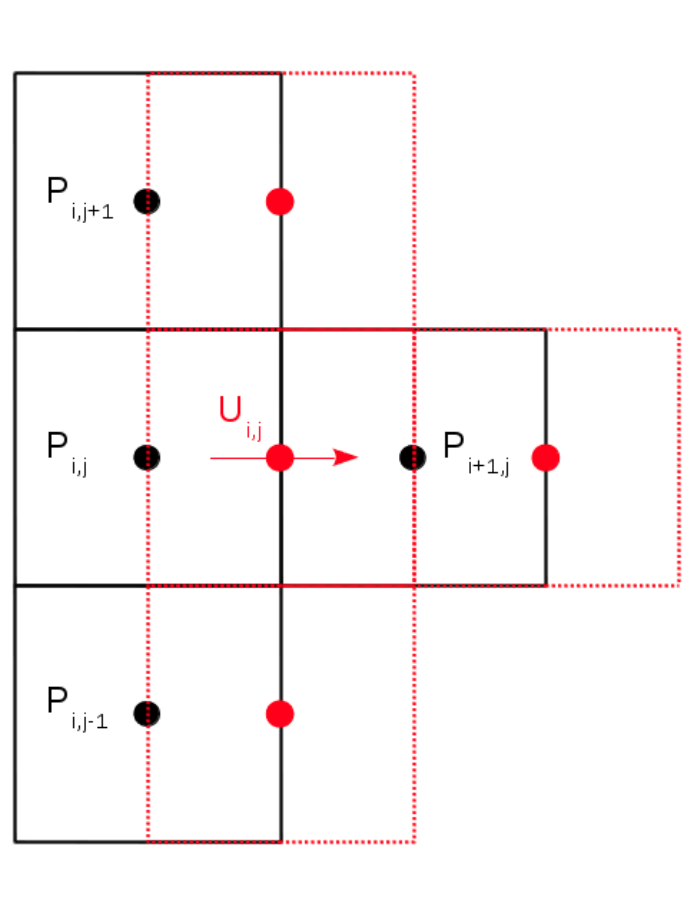
\includegraphics[width=\textwidth]{grilla_diferida_u.png}
      \caption{}
      \label{fig:grilla_desplazada_u}
  \end{subfigure}
  \hfill
  \begin{subfigure}[b]{0.2\textwidth}
      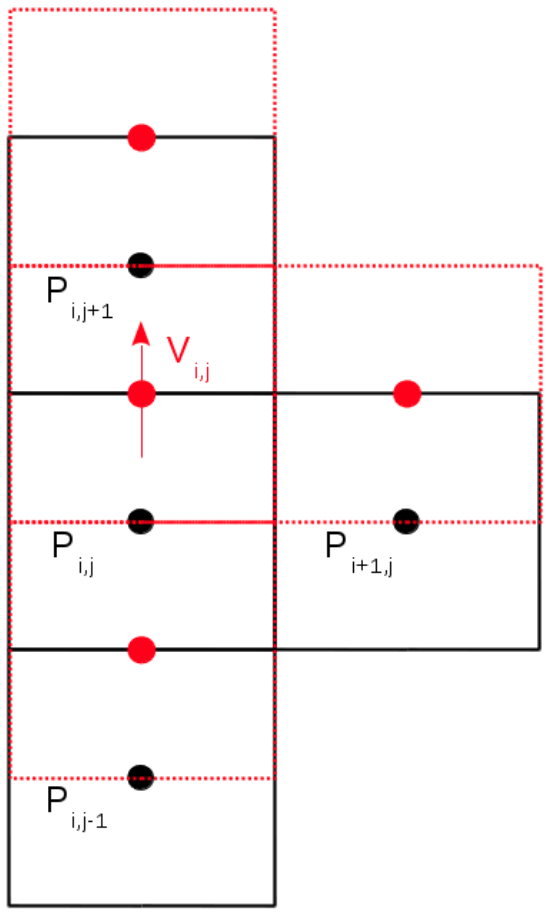
\includegraphics[width=\textwidth]{grilla_diferida_v}
      \caption{}
      \label{fig:grilla_desplazada_v}
  \end{subfigure}
     \caption{Esquema de las grillas desplazadas para la presión $p$ y las velocidades horizontal $u$ (\ref{fig:grilla_desplazada_u}) y vertical $v$ (\ref{fig:grilla_desplazada_v}). La grilla para $p$ es la única que posee todos sus volúmenes contenidos en la cavidad. Estas figuras fueron extraídas de \cite{Notas_materia}.}
     \label{fig:grillas_desplazadas}
\end{figure}


\ptitle{Discretización temporal}
Por otro lado, el dominio temporal se define desde $t = 0$ hasta $t = t_{max}$. El tiempo se discretizó en puntos equiespaciados $t_k = k \Delta t$ con $k = 0,1,\dots,M$ con $\Delta t = t_{max}/M$. De este modo, la presión $P_{ij}^k$ es la $P_{ij}$ evaluada en $t t_k$ y de forma análoga con las demás variables.


\subsection{Esquema numérico}

\ptitle{Resumen}
\begin{itemize}
  \item Se construyó un esquema numérico para las ecuaciones de conservación de momento \ref{eq:momento_x} y \ref{eq:momento_y} mediante la técnica de volúmenes finitos.
  \item Para aproximar los términos obtenidos se emplearon distintos métodos numéricos,analizando su efecto en la solución numérica.
  \item Para la evolución temporal se utilizó Euler Implícito y Crank-Nicolson
  \item Mientras que para el término advectivo se empleó diferencias centradas de orden 2, Up-wind de orden 1 y el \textcolor{red}{algoritmo?} QUICK. Por último, para el difusivo se empleó diferencias centradas de orden 2.
  \item Una vez planteado el esquema numérico, se resolvió el sistema de ecuaciones formado por \ref{eq:momento_x}, \ref{eq:momento_y} y \ref{eq:cons_masa} mediante el algoritmo SIMPLER.
  \item A continuación se explica la construcción del esquema numérico, junto a las características particulares de cada método utilzado.
\end{itemize}

\ptitle{Volúmenes finitos}
\begin{itemize}
  \item La implementación de la técnica de volúmenes finitos para este problema en particular se explica en detalle en \cite{Notas_materia}. 
  \item De forma resumida, se integran las ecuaciones de momento \ref{eq:momento_x} y \ref{eq:momento_y} en el volumen de las grillas de $u$ y $v$, respecticamente, empleando la regla del rectángulo \textcolor{red}{ref Moin}. Esta aproximación es de orden mayor a $\Delta^2$, correspondiente al mayor orden de aproximación de los esquemas para los términos advectivo y difusivo. De este modo se arriba a un sistema de ecuaciones donde el término temporal depende de $\partial U_{ij}/ \partial t$, el advectivo depende de $u$ evaluada en los cuatro laterales: $U_{N,ij}$ norte, $U_{S,ij}$ sur, $U_{E,ij}$ este y $U_{W,ij}$ oeste, y de $v$ evaluada de igual manera. Además, el término de presión depende de $P_{ij}$ y el término difusivo depende de las derivadas espaciales de $u$ evaluadas en los laterales: $\frac{\partial U_{E,ij}}{\partial x}$, $\frac{\partial U_{W,ij}}{\partial x}$, $\frac{\partial U_{N,ij}}{\partial y}$ y $\frac{\partial U_{S,ij}}{\partial y}$, y de las derivadas espaciales de $v$ de forma análoga.
  \item Es necesario aclarar que las variables anteriores se evalúan tanto en los laterales de los volúmenes de la grilla de $u$ como en los de $v$. Sin embargo, las aproximaciones para un caso y otro son análogas.
  \item En base a lo anterior, aplicar un método numérico determinado implica aproximar las velocidades $U_{ij}$, $V_{ij}$ y sus derivadas evaluadas en el centro y los laterales de sus volúmenes finitos respectivos.
  \item Por simetría $U_{E,ij} = U_{W,i+1j}$ y $U_{N,ij} = U_{S,ij+1}$. Además, cualquier aproximación sobre $U_{W,ij}$ vale sobre $U_{S,ij}$ intercambiando los índices $ij$ entre sí. De este modo, solo basta describir la aproximación en uno de los laterales
  \item Por último, una particularidad del término advectivo es su no linealidad, que se resuelve empleando la solución del paso previo como uno de los factores.
\end{itemize}


\ptitle{Métodos espaciales: presentación y aproximaciones para el término advectivo}
\begin{itemize}
  \item A continuación se desarrollan los métodos numéricos utilizados para el dominio espacial. Sólo se presentan las expresiones para la velocidad horizontal $u$, considerando que para la velocidad vertical $v$ son análogas.
  \item En cuanto al término advectivo, se empleron tres métodos numéricos: diferencias centradas de orden 2, Up-wind de orden 1 y \textcolor{red}{algoritmo?} QUICK.
  \item En diferencias centradas de orden 2 se aproxima
  \[U_{W,ij} = \frac{U_{ij} + U_{i-1j}}{2} \]
  \item Ventajas y desventajas
  \item En Up-wind de orden 1 se aproxima
  \[U_{W,ij} =  \left\{\begin{matrix}
    U_{i-1j} \qquad \mathrm{si} \qquad U_{W,ij}^*\geqslant 0\\
    U_{ij} \quad \qquad \mathrm{si} \qquad U_{W,ij}^* < 0
   \end{matrix}\right.\]
  \item donde el subíndice '*' indica que corresponde al paso previo o se calcula en base al paso previo.
  \item Ventajas y desventajas
  \item Por último, en \textcolor{red}{algoritmo?} QUICK se aproxima \textcolor{red}{REF}
  \[U_{W,ij} =  \left\{\begin{matrix}
    U_{i-1j} + \frac{1}{8}( - U_{i-2j} -2 U_{i-1j} + 3U_{ij} ) \, \qquad \mathrm{si} \qquad U_{W,ij}^*\geqslant 0\\
    U_{ij} + \frac{1}{8}(3 U_{i-1j} - 2 U_{ij} - U_{i+1j}) \quad \quad \qquad \mathrm{si} \qquad U_{W,ij}^* < 0
   \end{matrix}\right.\]
  \item ventajas y desventajas
\end{itemize}

\ptitle{Aproximaciones para el término difusivo}
\begin{itemize}
  \item En cuanto al término difusivo, se empleaon diferencis finitas centradas de orden 2:
  \[\frac{\partial U_{W,ij}}{\partial t} =  \frac{U_{ij} - U_{i-1j}}{\Delta}\]
  \item Ventajas y desventajas
\end{itemize}


\ptitle{Método de evolución temporal}
\begin{itemize}
  \item En cuanto a la evolución temporal, el sistema de ecuaciones discretizadas se puede llevar a uno de la forma
  \[\frac{\partial U_{ij}^k}{\partial t} = f(U^k,V^k,P^k)\]
  \[\frac{\partial V_{ij}^k}{\partial t} = g(U^k,V^k,P^k)\]
  donde $f$ y $g$ son funciones y $U^k$, $V^k$ y $P^k$ son las matrices de velocidad y presión evaluadas a tiempo $t = t_k$.
  \item En ambos casos la derivada temporal se aproximó mediante los métodos Euler Implícito y Crank-Nicholson. En el primero, se aproximó
  \[U_{ij}^{k+1} = U_{ij}^{k} + \Delta t f(U^{k+1},V^{k+1},P^{k+1})  + O_{local}({\Delta t}^2)\]
  y de forma análoga para $\frac{\partial V_{ij}^k}{\partial t}$.

  \item En el segundo, se aproximó
  \[U_{ij}^{k+1} = U_{ij}^{k} + \frac{\Delta t}{2} [f(U^{k+1},V^{k+1},P^{k+1}) + f(U^{k},V^{k},P^{k})] + O_{local}({\Delta t}^3).\]
  \item Este método implícito tiene la ventaja de tener factor de amplificación unitario.

\end{itemize}

\ptitle{Algoritmo simpler simplificadamente}
\begin{itemize}
  \item Mediante las aproximaciones anteriores, las ecuaciones de conservación de momento \ref{eq:momento_x} y \ref{eq:momento_y} se transforman en dos ecuaciones que sólo dependen de $U^k$, $U^{k-1}$, $V^k$, $V^{k-1}$, $P^k$ y $P^{k-1}$.
  \item Estas ecuaciones junto a la condición de divergencia libre \ref{eq:cons_masa} se resuelven mediante elalgoritmo SIMPLER. \cite{Patankar}
  \item Este es un algoritmo segregado o de paso fraccionado en el que se calculan por separado velocidad y presión. Partiendo de una aproximación de la velocidad y presión a tiempo $t_k$ es capaz de mejorarla mediante un método iterativo. Tal aproximación inicial suele ser la solución numérica a tiempo $t_{k-1}$. La exactitud de la solución depende del número de iteraciones internas $l_{simpler}$ realizadas, a expensas de un mayor costo computacional.
\end{itemize}



\subsection{Costo computacional}

\ptitle{Costo computacional y elección de $n$}
Debido a la cantidad de variables involucradas, proporcional a $n^2$, y dependiendo del número de pasos de tiempo a realizar, el costo computacional puede ser alto. En base a esto, es importante desarrollar métodos que permitan disminuir el costo pero que a su vez tengan una precisión aceptable. Un modo de minimizarlo es disminuyendo el número de variables pero exigiendo a su vez un error menor al 5 \%, por ejemplo. Sin embargo, para esto es necesario conocer la solución exacta o al menos una muy buena aproximación, lo cual no siempre se tiene.

\ptitle{Elección de $M$}
Otra alternativa es disminuyendo el número de pasos de tiempo $M$. Cuando $U_0(t)$ es independiente del tiempo, el sistema de ecuaciones REFs debe llegar a un estado estacionario a partir del cual la solución deja de variar. Una vez en este estado, no tiene sentido continuar la ejecución. Entonces, se puede aplicar un criterio de convergencia que para dado $\Delta t$ indique cuándo la solución se encuentra en el estado estacionario y la ejecución debe detenerse. El criterio tomado fue el siguiente: si la solución tiende a un estacionario independiente del tiempo, entonces se avanza la solución hasta que se cumplan al mismo tiempo las desigualdades
\[\frac{\left \|U^{k+1}-U^k \right \|_2}{\Delta t} < tol, \, \frac{\left \| V^{k+1} - V^k \right \|}{dt} < tol \]
con $tol$ tolerancia. A menor $tol$, mayor el costo computacional debido a que se necesitan más pasos $M$. En este trabajo se decidió establecer $tol = 1 \times 10^{-5}$.
\ptitle{Algoritmo para $\Delta t$}

Además, si solo es de interés la solución en el estado estacionario, otra alternativa es eligir $\Delta t$ de modo que la solución converja más rápido a pesar de tener un estado transitorio lejos de la solución exacta. Esto último se basa en la hipótesis de que la solución no depende del paso de tiempo, lo cual debe ser estudiado en detalle. Asumiendo que así es, se propone el siguiente algoritmo para elegir $\Delta t$.
\begin{enumerate}
  \item Se parte de una propuesta $\Delta t_{guess}$ lo suficientemente pequeña para que asegurar que la solución no diveja. En este trabajo se empleó $\Delta t_{guess} = 0.005.$ 
  \item Se avanza en 10 pasos la solución numérica, calculando en cada uno de ellos el parámetro $\epsilon$ definido como
  \[\epsilon = \sqrt{ \left \|U^{k+1}-U^k \right \|_2^2 +  \left \| V^{k+1} - V^k \right \|_2^2 }.\]
  Este parámetro da indicio de cuán rápido varían las velocidades.
  \item Se calcula la velocidad de convergencia $\chi_{guess}$ definida como la pendiente en un ajuste lineal de $\ln{\epsilon}$ vs número de paso de tiempo.
  \item Se divide el paso de tiempo por la mitad $\Delta t = \Delta t_{guess}/2$ y se calcula la velocidad de convergencia $\chi$ correspondiente. Si $\chi > \chi_{guess}$, se divide el paso de tiempo por la mitad y se repite el proceso empleando $ \Delta t_{guess} = \Delta t$. Si $\chi < \chi_{guess}$, se define determina como mejor paso de tiempo a $\Delta t_{guess}$.
\end{enumerate}


\ptitle{Número de pasos $l_{simpler}$}
\begin{itemize}
  \item Por último, a mayor $l_{simpler}$, mayor exactitud del método SIMPLER y mayor costo computacional. De este modo, suena lógico mantener $l_{simpler} = 1$. Sin embargo, como cambia la precisión del método, podría modificarse también la elección de $\Delta t$ y, consecuentemente, aumentar o disminuir el número de pasos de tiempo $M$ necesarios para llegar al estado estacionario
  \item En definitiva, la relación entre $l_{simpler}$ y costo computacional podría no ser trivial y debe ser estudiada en detalle.
\end{itemize}


\ptitle{Resumen de costo computacional}
En este trabajo se estudiaron todos los métodos mencionados. En primer lugar, se determinó para $Re = 100$ y $1000$, el valor de $n_1$ tal que la solución numérica tiene un error menor al 5 \% respecto a una solución numérica de mayor precisión obtenida en \textcolor{red}{ref Guia}. En segundo lugar, estudiando la velocidad de convergencia en función de $\Delta t$ se planteó un algoritmo que permita elegir $\Delta t$ de modo de minimizar el número de pasos de tiempo necesarios. En tercer lugar, se decidió emplear el criterio de elección de $M$ durante todo el trabajo.

\ptitle{Resumen de lo que se va a estudiar}
\begin{itemize}
  \item En primer lugar, se estudió la dependencia de la solución en el estado estacionario con respecto al paso temporal.
  \item Se planteó un algoritmo para minimizar el costo computacional para encontrar el estado estacionario con un error menor al 5 \%
  \item Se evaluó el efecto de los pasos internos del algoritmo simpler
  \item En segundo lugar, se estudió el impacto en el estacionario del esquema espacial en el término advectivo empleando distintos números de Reynolds. En particular, se utilizaron diferencias centradas de orden 2, Up-wind de orden uno y el esquema QUICK de orden \textcolor{red}{?}
  \item Además, se estudió el orden de convergencia espacial de Up-wind de primer orden en referencia al mejor esquema advectivo
  \item Se estudió el efecto del método de evolución temporal, evaluando el estado transitorio de la solución mediante los métodos Euler Implícito y Crank-Nicholson
\end{itemize}



\section{Resultados y discusión}


\subsection{Dependencia del estado estacionario con el paso dt}

En primer lugar, se analizó la dependencia del estado estacionario con el paso de evolución temporal. El estado estacionario se define en base al criterio de convergencia descripto en la sección anterior con una tolerancia $tol = 1 \times 10^{-5}$. Se calculó $u(0.5,0.5)$ y $v(0.5,0.5)$ para $Re = 1000$, $n = 20$, $l_simpler = 1$ y distintos $\Delta t$ entre $0.005$ y $20$. Se emplearon diferencias centradas de orden 2 para el término advectivo y Euler implícito para la evolución temporal. En la figura \ref{fig:a_vel_vs_dt} se grafican $\delta u(0.5,0.5)$ y $\delta v(0.5,0.5)$ definidos como la diferencia en valor absoluto entre la velocidad con determinado $\Delta t$ y su valor con $\Delta t = 0.005$. Se observa una diferencia entre los valores obtenidos del orden de $1 \times 10^{-4}$, ligeramente superior a la tolerancia en el criterio de convergencia. Aunque si solo se consideraran $\Delta t \lessim 1$, se obtendría una diferencia menor a dicha tolerancia y por lo tanto se podría decir que el estado estacionario no depende de $\Delta t$. De este modo, bajo estas condiciones es válido el uso del algortimo para calcular el mejor $\Delta t$ descripto en la sección anterior. Si bien la afirmación anterior sólo es válida en el caso particular considerado, se tomará como normal general en próximas simulaciones.

\textcolor{red}{Incluso lo voy a tomar independiente directamente de $\Delta t$ sin importar el rango. ¿Qué significa que sea independiente de delta t? Puede tener un transitorio lejos del exacto pero un estacionario idéntico}

\begin{figure}[h]
  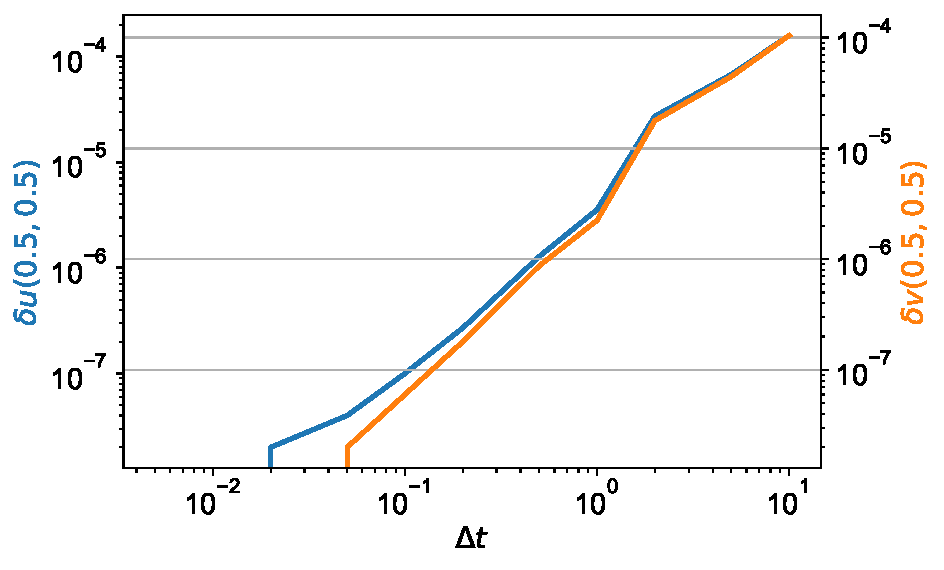
\includegraphics[clip=true,width=\columnwidth]{a_vel_vs_dt.pdf}
  \caption{$\delta u(0.5,0.5)$ y $\delta v(0.5,0.5)$ en función del paso temporal $\Delta t$. Se empleó $Re = 1000$, $n = 20$ y $l_{simpler} = 1$. Además, se utilizó diferencias finitas centradas de orden 2 para el término advectivo y difusivo y Euler implícito para la evolución temporal.}
   \label{fig:a_vel_vs_dt}
\end{figure}


\subsection{Costo computacional}

\ptitle{Resumen}
\begin{itemize}
  \item El algoritmo para encontrar el mejor $\Delta t$ permite disminuir el número de pasos necesarios para alcanzar el estado estacionario, lo cual disminuye a su vez el costo computacional.
  \item Otro modo de hacer esto último es reduciendo el número de variables involucradas. En este caso se debe tener cuidado de no perder precisión en la solución, para lo cual es útil tener una solución de referencia con mayor precisión. En este trabajo se empleó la solución numérica de \textcolor{red}{ref guia} como referencia.
  \item Para encontrar el mínimo $n$ se empleó el siguiente algoritmo. Se comenzó con $n = 30$, lo suficientemente grande para asegurar un error menor al 5 \%. Luego, se redujo $n$ en dos unidades, se avanzó la solución hasta el estado estacionario eligiendo $\Delta t$ mediante el algoritmo presentado en la sección anterior y se midió el error. Si este es menor al 5 \% se disminuye nuevamente $n$. Si es mayor al 5 \%, se define como el mejor valor de $n$ al valor anterior.
  \item Se observó el efecto de ambos algoritmos en casos particulares. Para $Re = 100$ y $1000$ se midió el tiempo de cómputo $T$ para encontrar $u(0.5,0.5)$ en el estado estacionario con un error menor al 5 \%.
  \item Se empleó DC2 para el término difusivo y UP1 y DC2 para el advectivo. Para la evolución temporal se empleó EI.
  \item Los resultados se resumen en la tabla \ref{tabla:costo_computacional}
  \item Se 
\end{itemize}


\begin{table}[]
  \begin{tabular}{|c|c|c|c|c|c|}
  \hline
  \begin{tabular}[c]{@{}c@{}}método para el\\ termino advectivo\end{tabular} & $Re$ & $n$ & $\Delta t$ & $N$ & $T [min]$ \\ \hline
  DC2 & 100 & 20 & 2.56 & 22 & 4.5 \\ \hline
  UP1 & 100 & 32 & 1.28 & 25 & 0.9 \\ \hline
  DC2 & 1000 & 30 & 0.16 & 768 & 11.3 \\ \hline
  UP1 & 1000 & 32 & 5.12 & 59 & 1.2 \\ \hline
  \end{tabular}
  \label{tabla:costo_computacional}
  \caption{Test}
\end{table}


% \ptitle{Para qué se usó el algoritmo anterior}
% \begin{itemize}
%   \item Este algoritmo no siempre va a encontrar el mejor $\Delta t$ posible, pero se espera que esté cerca del óptimo.
%   \item El algoritmo anterior fue empleado para hallar el estado estacionario en todo este trabajo salvo el caso particular $n_1 = 80$. Este es el caso más costoso y se buscará a mano el mejor $\Delta t$ para cada $Re$ específico.
%   \item Se usaron $\Delta t = 0.35$, $1.25$ y $2.0$ para $Re = 100$, $1000$ y $5000$, respecticamente
% \end{itemize}

\subsection{dt para distintos lsimpler}

\begin{itemize}
  \item Se estudió la dependencia del paso de tiempo y del costo computacional en función del número de iteraciones internas del algoritmo $l_{simpler}$
  \item Para representar el costo computacional se utilizó el tiempo $T$ necesario para que se encuentre el mejor $\Delta t$ y se llegue al estado estacionario.
  \item Se emplearon las mismas condiciones que en la simulación anterior a excepción del número de volúmenes finitos $n = 30$.
  \item Los resultados se resumen en la tabla \ref{dt_costo_vs_lsimpler}
  \item Se observa que el número de pasos de tiempo necesarios para alcanzar el estado estacionario varía ligeramente con $l_{simpler}$, no así el tiempo de cómputo que aumenta de forma proporcional con el mismo. Por otro lado, el valor de $\Delta t$ calculado mediante el algoritmo es independiente de $l_{simpler}$.
  \item La información anterior da idea del costo computacional pero cabe preguntarse cómo cambia la precisión con $l_{simpler}$. En la figura \ref{fig:lsimpler} se grafican las velocidades $u(0.5,y)$ y $v(x,0.5)$ en el estado estacionario para los distintos valores de $l_simpler$.
  \item Cualitativamente, las velocidades en el estado estacionario no se modifican con $l_{simpler}$. Sin embargo, la solución numérica dista de la de referencia. Esto podría deberse al valor de $n$ utilzado o a los métodos numéricos en sí.
\end{itemize}

\begin{figure}[h]
  \includegraphics[clip=true,width=\columnwidth]{dt_costo_vs_lsimpler.pdf}
  \caption{}
   \label{fig:dt_costo_vs_lsimpler}
\end{figure}

\begin{figure}
  \centering
  \begin{subfigure}[b]{0.3\textwidth}
      \centering
      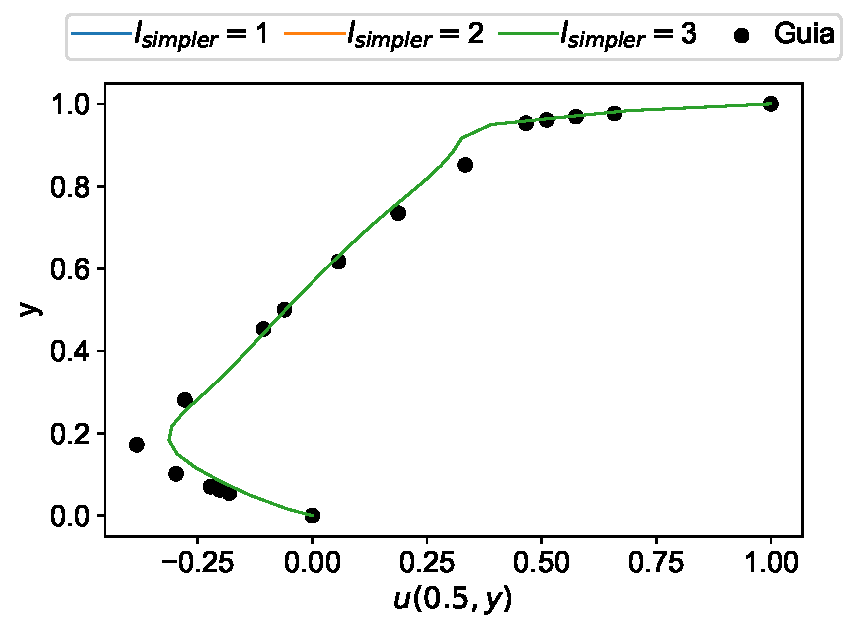
\includegraphics[width=\textwidth]{f_lsimpler_u.pdf}
      \caption{}
      \label{fig:lsimpler_u}
  \end{subfigure}
  \hfill
  \begin{subfigure}[b]{0.3\textwidth}
      \centering
      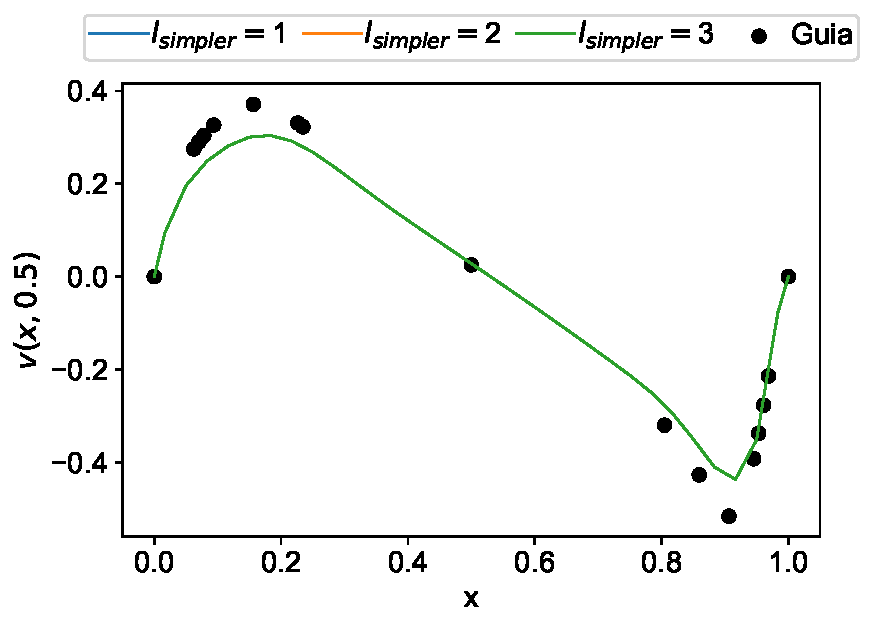
\includegraphics[width=\textwidth]{f_lsimpler_v.pdf}
      \caption{}
      \label{fig:lsimpler_v}
  \end{subfigure}
     \caption{Velocidades $u(0.5,y)$ y $v(x,0.5)$ en el estado estacionario para $l_simpler = 1$, $2$ y $3$ iteraciones internas en el algoritmo SIMPLER. En ambos casos todas las curvas están superpuestas. Se empleó $Re = 1000$ y $n = 30$. Además, se utilizó diferencias finitas centradas de orden 2 para el término advectivo y difusivo y Euler implícito para la evolución temporal.}
     \label{fig:lsimpler}
\end{figure}

\begin{table}[]
  \begin{tabular}{|c|c|c|c|}
  \hline
  \multicolumn{1}{|c|}{$l_{simpler}$ \quad} & \multicolumn{1}{c|}{$N$\quad} & \multicolumn{1}{c|}{$\Delta t$\quad} & \multicolumn{1}{c|}{$T [min]$} \\ \hline
  1 & 756 & 0.16 & 5.8 \\ \hline
  2 & 793 & 0.16 & 12.7 \\ \hline
  3 & 800 & 0.16 & 18.8 \\ \hline
  \end{tabular}
  \label{tabla:dt_costo_vs_lsimpler}
  \caption{test}
\end{table}

Hay que estudiar en detalle la dependencia de la solución con los métodos numéricos para el término advectivo y la evolución temporal


\subsection{Término advectivo}

\textcolor{red}{Los captions no están siendo autocontenidos. Hay que mencionar qué curva se encima sobre cuál}

Se estudió en detalle el comportamiento de la solución con el método numérico empleado para el término advectivo. Se implementaron los esquemas DC2, UP1 y QUICK y se calculó el estado estacionario para $Re = 100, 1000 \, \mathrm{y} \, 5000$, para $n1 = 20, 40 \, \mathrm{y} \, 80$ y para los tres esquemas mencionados. Se empleó DC2 para el término difusivo y Euler implícito para la evolución temporal.

\ptitle{Comparación DC2 vs n1 para distintos Re}
En primer lugar, se estudió la dependencia del estado estacionario con la discretización espacial $n$ y el número de $Re$, empleando DC2 para el término advectivo
\begin{itemize}
  \item En las figuras \ref{fig:velocidades_u_DC2_vs_Re} y \ref{fig:velocidades_v_DC2_vs_Re} se grafican las velocidades $u(0.5,y)$ y $v(x,0.5)$ para los distintos casos.
  \item Para $Re = 100$ se observa que el resultado varía cualitativamente poco con el tamaño de la discretización.
  \item Para $Re = 1000$ la diferencia entre los resultados es significativa, llegando en algunos sitios a superar la tolerancia de $1 \times 10^{-5}$ del criterio de convergencia.
  \item Por último, para $Re = 5000$ todas las soluciones distan de la referencia.
  \item Esto indica que a mayor número de Reynolds es necesario disminuir el tamaño de la discretización, es decir, aumentar $n_1$, para obtener una solución más precisa. \textcolor{red}{No justifico porque no sé justificar}
\end{itemize}

\ptitle{Comparación cualitativa entre métodos numéricos para distintos Re}
En segundo lugar, se estudió la dependencia del estado estacionario con el número de Reynolds y el método numérico para el término advectivo. En todos los casos se empleó $n = 80$.

\begin{itemize}
  \item En las figuras \ref{terminos_advs_u} y \ref{terminos_advs_u} se grafica la velocidad $u(0.5,y)$ y $v(x,0.5)$ para los distintos casos. 
  \item Cualitativamente, para $Re = 100$ no se observan grandes diferencias.
  \item Para $Re = 1000$ es notable que el método UP1 no aproxima correctamente la solución, mientras que DC2 y QUICK sí lo hacen. Esto se puede justificar en los órdenes de aproximación de los métodos, siendo el primero de orden 1 y los segundos de orden 2 \textcolor{red}{QUICK es orden 2? Hacer la cuenta}
  \item Para $Re = 5000$ ninguno de los métodos aproxima correctamente la solución en la totalidad del dominio. En base a los resultados obtenidos al variar $n$, esto podría deberse al tamaño de la grilla espacial y no al método numérico.
  \item Cabe preguntarse por qué a medida que aumenta $Re$ la solución con UP1 se aleja aún más de la de referencia. A mayor $Re$, el término advectivo en las ecuaciones de momento \ref{eq:momento_x} y \ref{eq:momento_y} gana imporancia respecto al difusivo. De este modo, se esperaría una solución con baja difusión. Sin embargo, el método UP1 presenta naturalmente difusión y de este modo la solución numérica se aparta de la referencia.
\end{itemize}

\ptitle{Comparación numérica entre métodos numéricos para distintos $Re$.}
Para cada variación posible de $n_1$, $Re$ y método para el término advectivo, se calculó el error relativo $e_{rel}$ respecto a la bibliografía \textcolor{red}{referencia a GUIA} en el centro del dominio $x = 0.5$ e $y = 0.5$. Para calcular este error se suman cuadráticamente los errores en $u$ y $v$ y se normaliza con el valor de referencia, es decir,
\[e_{rel} = \frac{\sqrt{(u_{exp} - u_{sol})^2 + (v_{exp} - v_{sol})^2}}{\sqrt{u_{sol}^2 + v_{sol}^2}}. \]
donde todos las velocidades están evaluadas en el centro


% Mencionar cómo se calcula $u(0.5,0.5)$ y que sólo tiene sentido calcularlo allí porque la aproximación es del mismo orden que los métodos. Calcularla en otro lado con un promedio ponderado es de mayor orden.



\begin{itemize}
  \item Para calcular las velocidades en el centro se promediaron los valores en la cercanía, resultando en una aproximación de segundo orden.
  \item Los resultados se resumen en la figura \ref{fig:termino_advectivo}.
  \item Al comportamiento visto en las figuras \ref{terminos_advs_u} y \ref{terminos_advs_u} se agregan dos particularidades. En primer lugar, independientemente de $Re$ el método UP1 presenta mayor error que los demás, lo cual es esperable por ser un método de menor orden. En segundo lugar, en casi todos los casos a mayor $n$, menor error. La excepción son los casos de $Re = 100$, $n = 80$ y DC2 y QUICK como método para el término advectivo. \textcolor{red}{por qué será?}

  \item Por último, cabe preguntarse qué método es más preciso. Para tal fin se resumen en la tabla \ref{tabla:erel} los errores de cada método para $n = 80$ y $Re = 100$, $1000$ y $5000$. Se observa que el método DC2 posee un error ligeramente menor a QUICK. Entonces, se podría argumentar que DC2 es un método más preciso que QUICK. Sin embargo, esta afirmación debe tomarse con cuidado debido a que sólo se analizó la velocidad en el punto central y no en todo el dominio. En un análisis formal podría obtenerse el comportamiento opuesto.
\end{itemize}




\onecolumngrid


\begin{figure}
  \centering
  \begin{subfigure}[b]{0.32\textwidth}
      \centering
      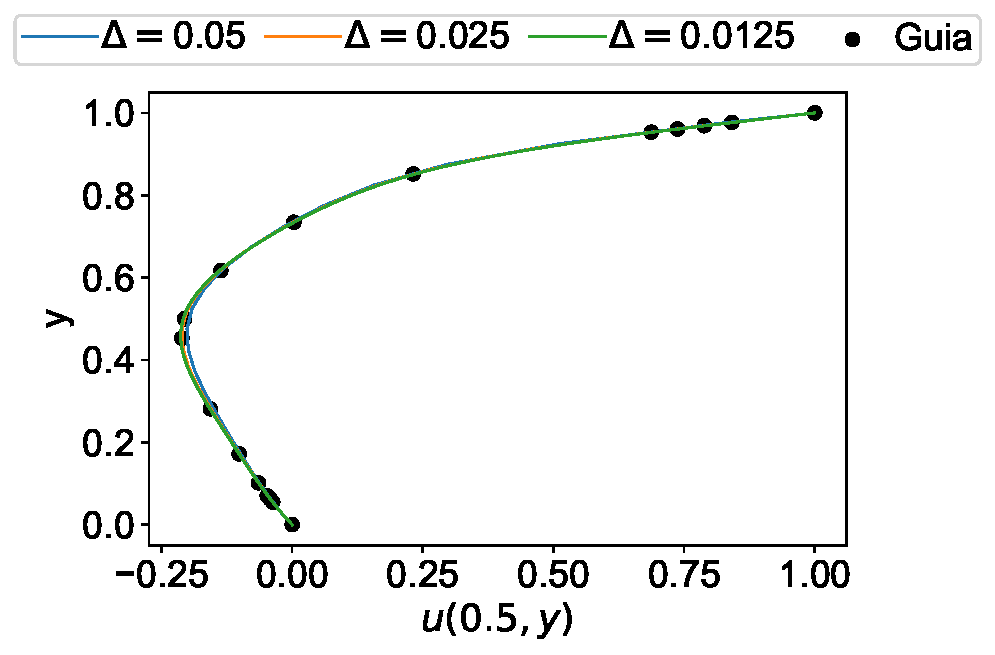
\includegraphics[width=\textwidth]{termino_adv_Db_u_100.pdf}
      \caption{}
      \label{fig:termino_adv_Db_u_100}
  \end{subfigure}
  \hfill
  \begin{subfigure}[b]{0.32\textwidth}
      \centering
      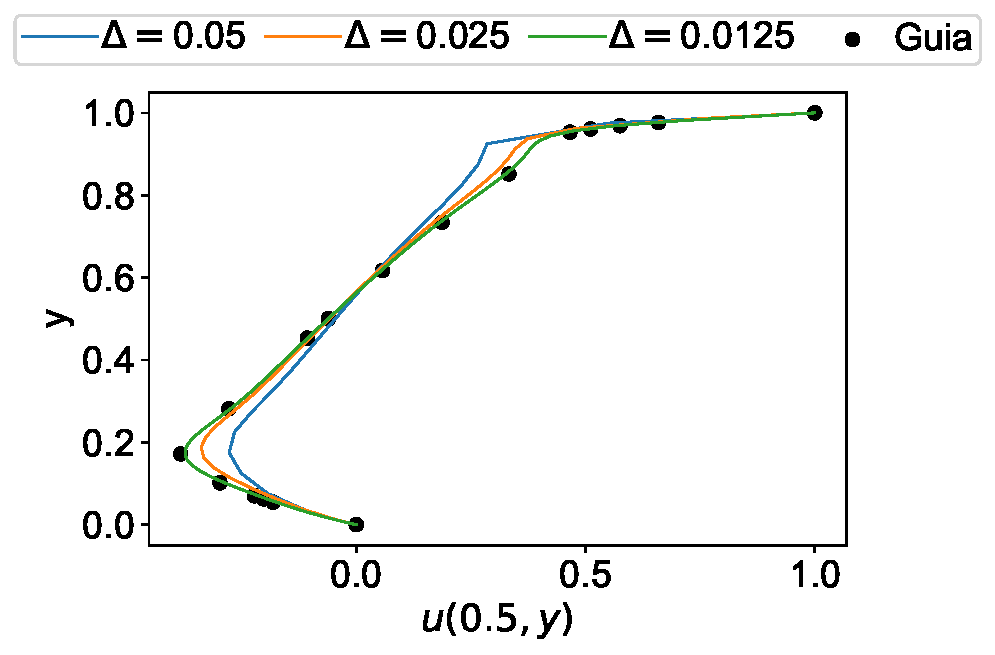
\includegraphics[width=\textwidth]{termino_adv_Db_u_1000.pdf}
      \caption{}
      \label{fig:termino_adv_Db_u_1000}
  \end{subfigure}
  \hfill
  \begin{subfigure}[b]{0.32\textwidth}
      \centering
      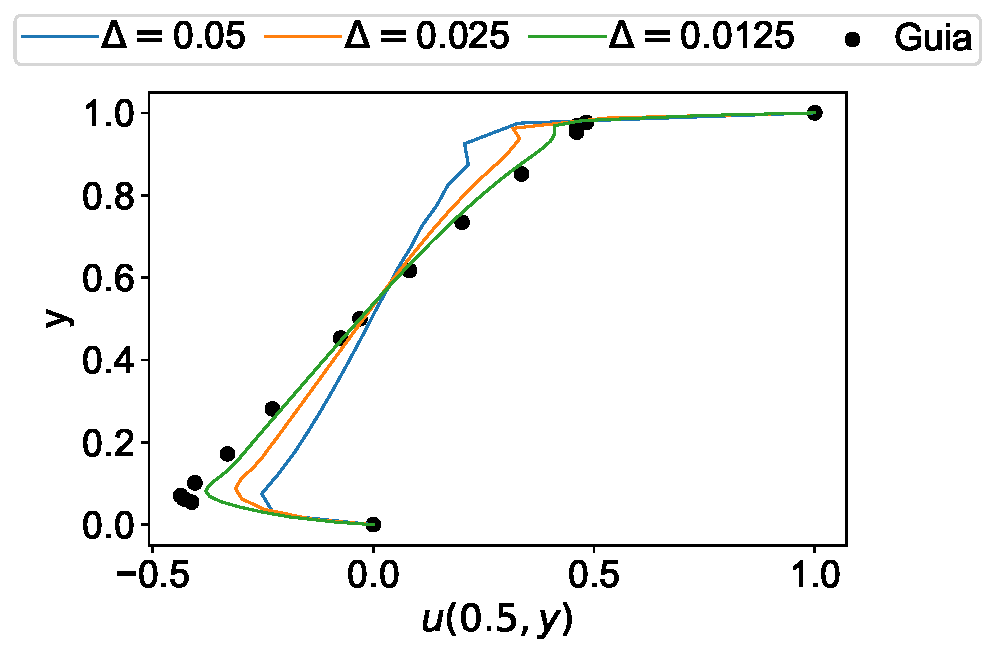
\includegraphics[width=\textwidth]{termino_adv_Db_u_5000.pdf}
      \caption{}
      \label{fig:termino_adv_Db_u_5000}
  \end{subfigure}
     \caption{Velocidad $u(0.5,y)$ en el estado estacionario en función de $y$ para distinto tamaño de la discretización espacial $\Delta$ y número de Reynolds $Re$: (a) $Re = 100$, (b) $Re = 1000$ y (c) $Re = 5000$.}
     \label{fig:velocidades_u_DC2_vs_Re}
\end{figure}

\begin{figure}
  \centering
  
  \begin{subfigure}[b]{0.32\textwidth}
    \centering
    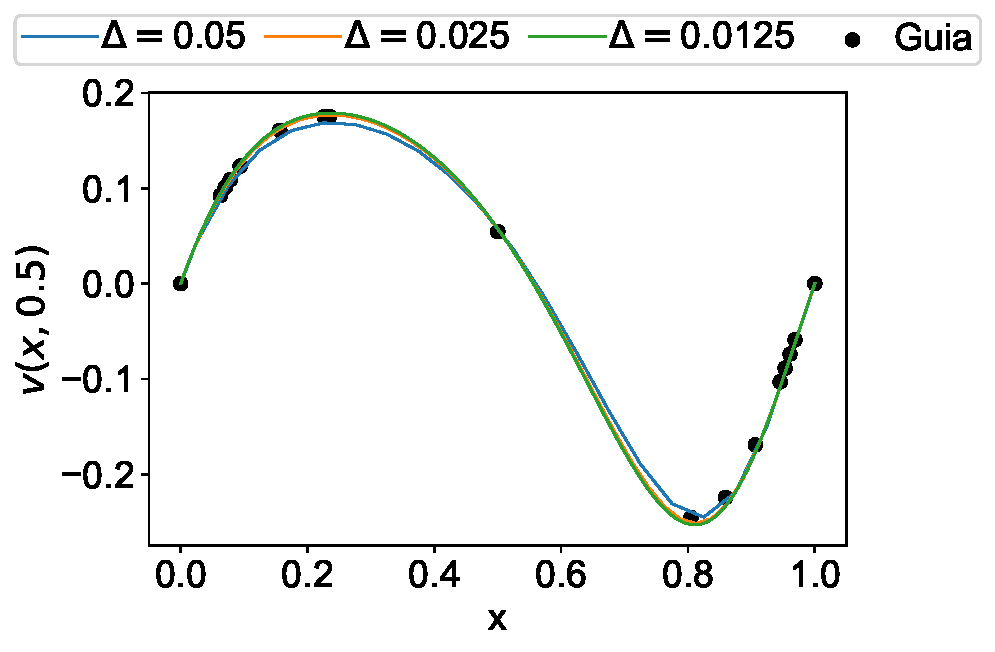
\includegraphics[width=\textwidth]{termino_adv_Db_v_100.pdf}
    \caption{}
    \label{fig:termino_adv_Db_v_100}
\end{subfigure}
\hfill
\begin{subfigure}[b]{0.32\textwidth}
    \centering
    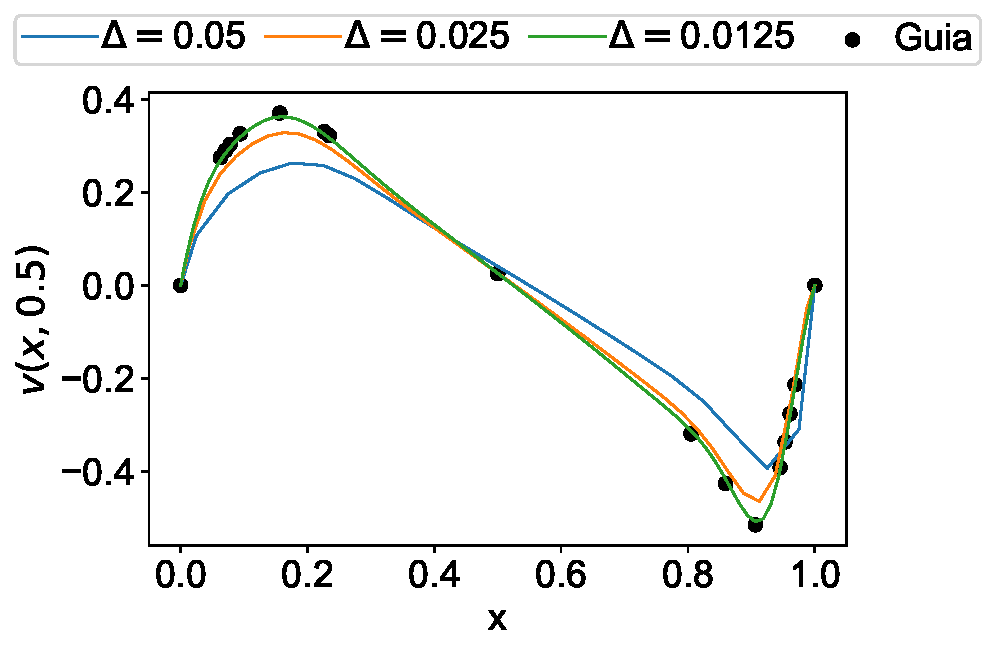
\includegraphics[width=\textwidth]{termino_adv_Db_v_1000.pdf}
    \caption{}
    \label{fig:termino_adv_Db_v_1000}
\end{subfigure}
\hfill
\begin{subfigure}[b]{0.32\textwidth}
    \centering
    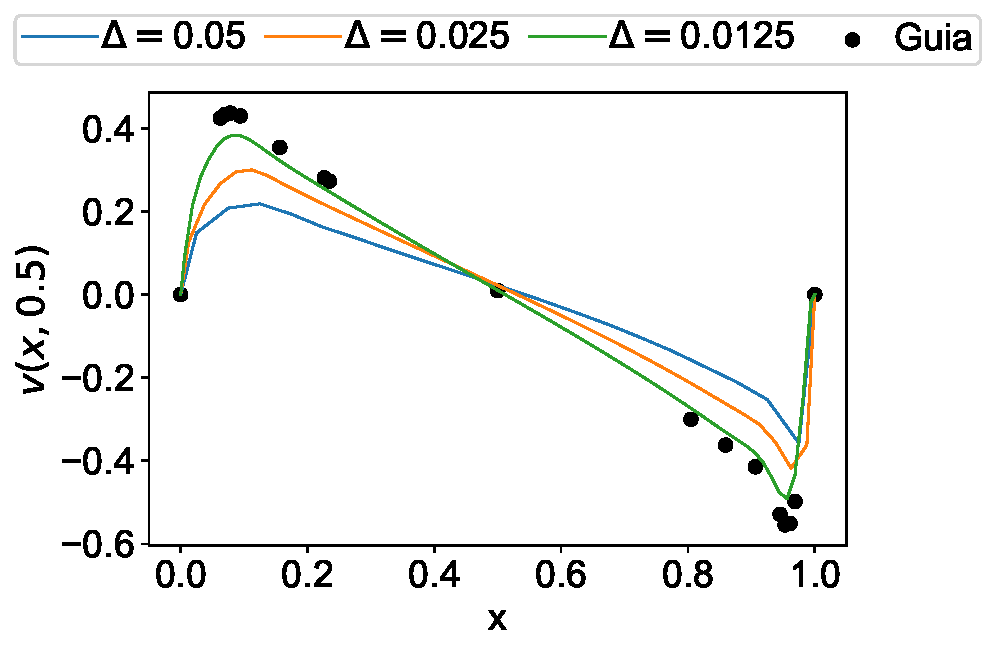
\includegraphics[width=\textwidth]{termino_adv_Db_v_5000.pdf}
    \caption{}
    \label{fig:termino_adv_Db_v_5000}
\end{subfigure}
     \caption{Velocidad $v(x,0.5)$ en el estado estacionario en función de $x$ para distinto tamaño de la discretización espacial $\Delta$ y número de Reynolds $Re$: (a) $Re = 100$, (b) $Re = 1000$ y (c) $Re = 5000$.}
     \label{fig:velocidades_v_DC2_vs_Re}
\end{figure}






\begin{figure}
  \centering
  \begin{subfigure}[b]{0.32\textwidth}
      \centering
      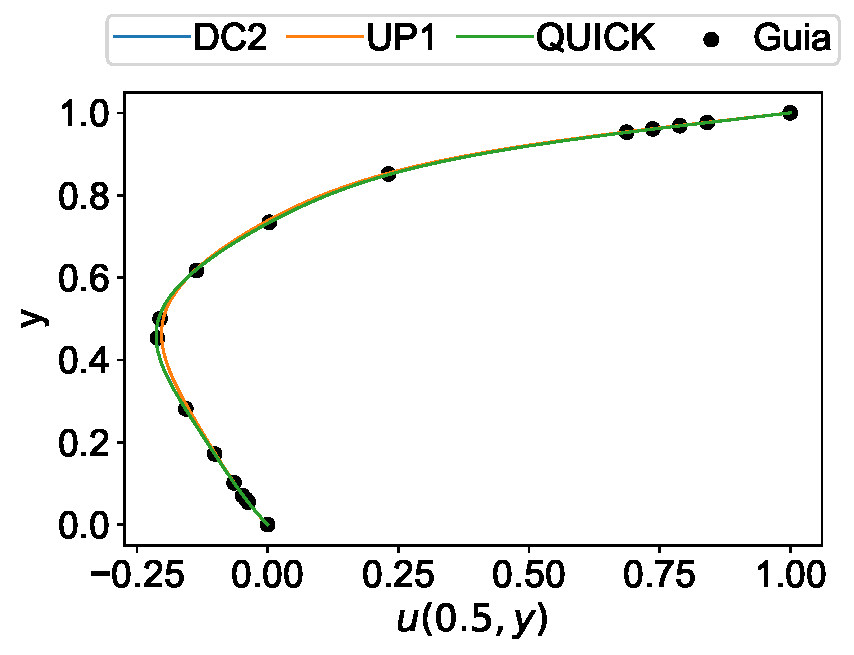
\includegraphics[width=\textwidth]{terminos_advs_u_100.pdf}
      \caption{}
      \label{fig:terminos_advs_u_100}
  \end{subfigure}
  \hfill
  \begin{subfigure}[b]{0.32\textwidth}
      \centering
      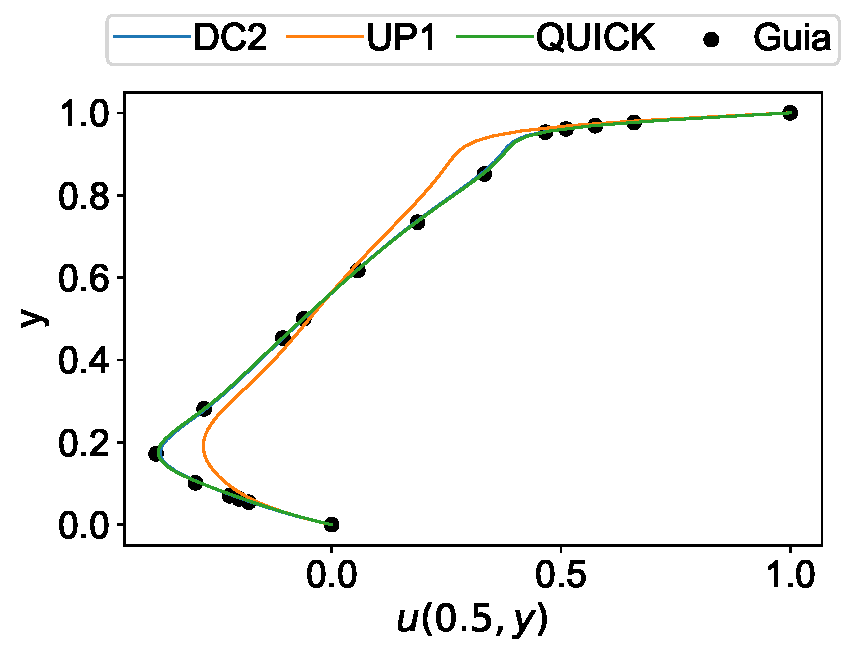
\includegraphics[width=\textwidth]{terminos_advs_u_1000.pdf}
      \caption{}
      \label{fig:terminos_advs_u_1000}
  \end{subfigure}
  \hfill
  \begin{subfigure}[b]{0.32\textwidth}
      \centering
      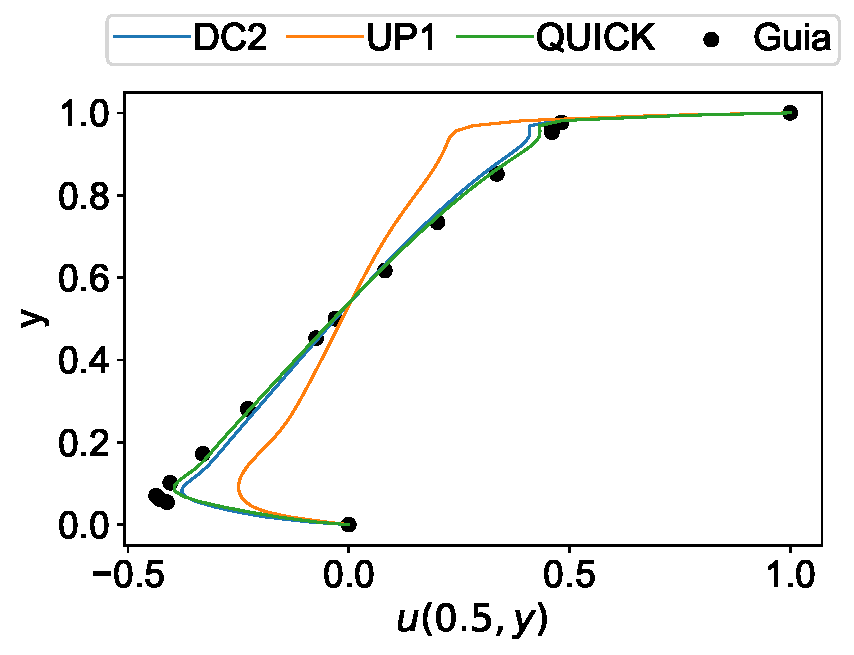
\includegraphics[width=\textwidth]{terminos_advs_u_5000.pdf}
      \caption{}
      \label{fig:terminos_advs_u_5000}
  \end{subfigure}
     \caption{Velocidad $u(0.5,y)$ en el estado estacionario en función de $y$ para distintos métodos numéricos para el término advectivo y distintos números de Reynolds $Re$: (a) $Re = 100$, (b) $Re = 1000$ y (c) $Re = 5000$. En todos los casos se empleó una grilla espacial de tamaño $n_1 \times n_1$ con $n_1 = 80$, diferencias centradas de orden 2 para el término difusivo y Euler implícito para la evolución temporal.}
     \label{fig:terminos_advs_u}
\end{figure}

\begin{figure}
  \centering
  \begin{subfigure}[b]{0.32\textwidth}
    \centering
    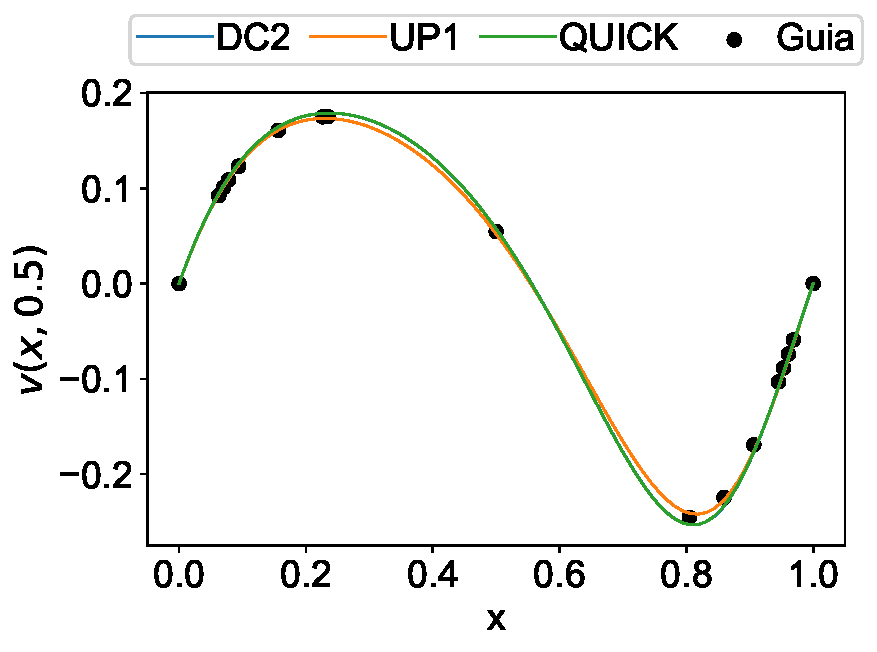
\includegraphics[width=\textwidth]{terminos_advs_v_100.pdf}
    \caption{}
    \label{fig:terminos_advs_v_100}
  \end{subfigure}
  \hfill
  \begin{subfigure}[b]{0.32\textwidth}
    \centering
    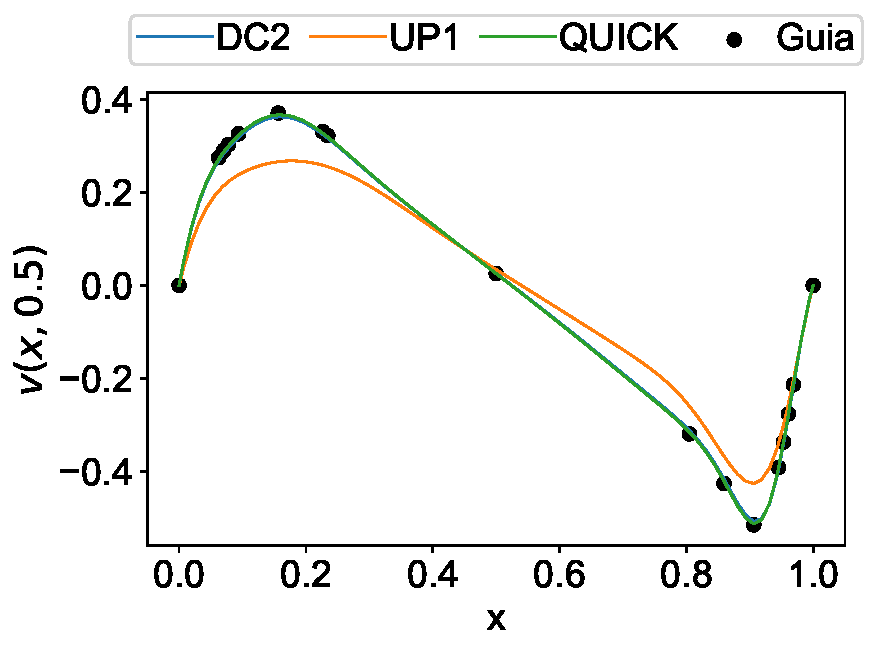
\includegraphics[width=\textwidth]{terminos_advs_v_1000.pdf}
    \caption{}
    \label{fig:terminos_advs_v_1000}
  \end{subfigure}
  \hfill
  \begin{subfigure}[b]{0.32\textwidth}
    \centering
    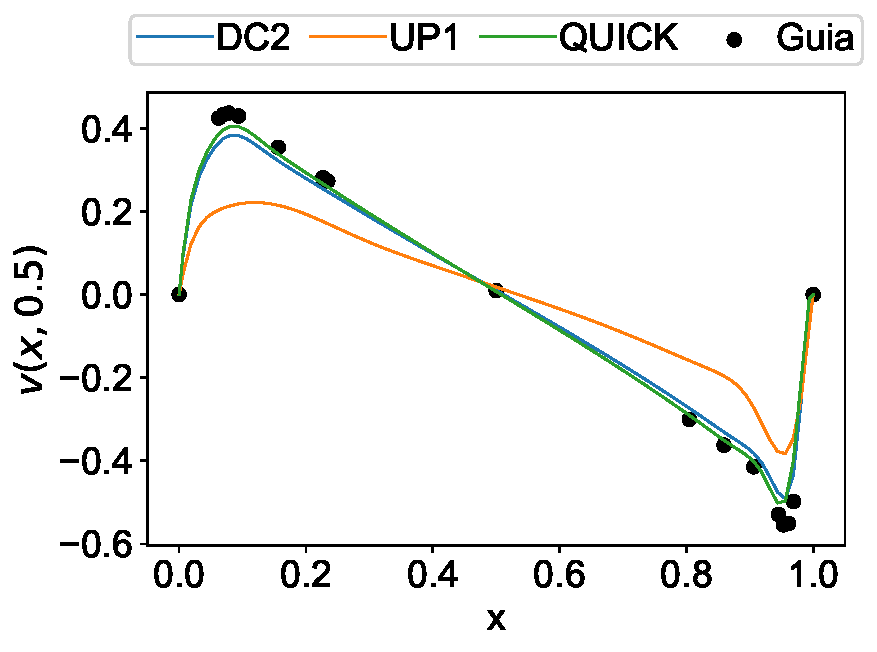
\includegraphics[width=\textwidth]{terminos_advs_v_5000.pdf}
    \caption{}
    \label{fig:terminos_advs_v_5000}
  \end{subfigure}
     \caption{Velocidad $v(x,0.5)$ en el estado estacionario en función de $x$ para distintos métodos numéricos para el término advectivo y distintos números de Reynolds $Re$: (a) $Re = 100$, (b) $Re = 1000$ y (c) $Re = 5000$. En todos los casos se empleó una grilla espacial de tamaño $n_1 \times n_1$ con $n_1 = 80$, diferencias centradas de orden 2 para el término difusivo y Euler implícito para la evolución temporal.}
     \label{fig:terminos_advs_v}
\end{figure}



\begin{figure}
  \centering
  \begin{subfigure}[b]{0.32\textwidth}
      \centering
      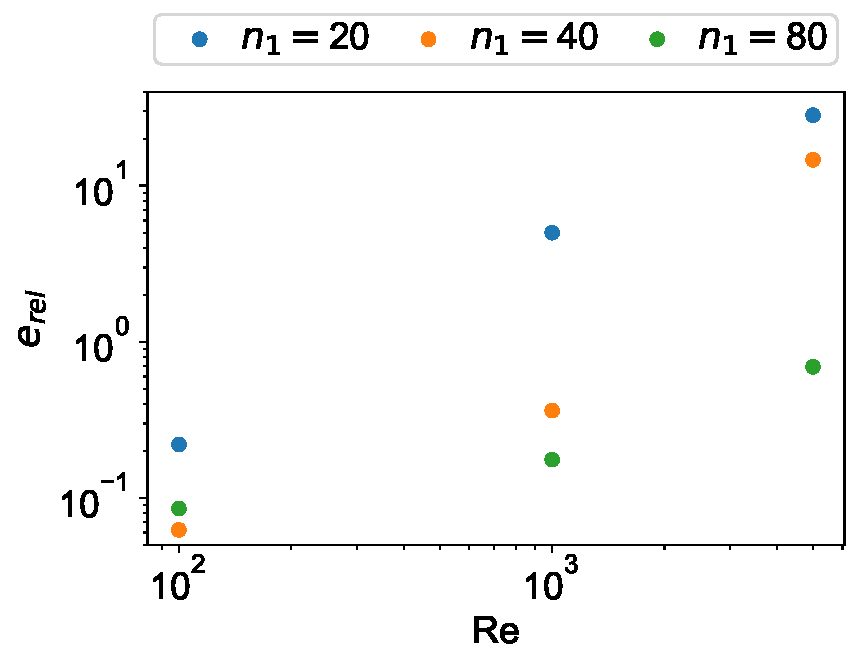
\includegraphics[width=\textwidth]{termino_adv_DC2.pdf}
      \caption{}
      \label{fig:termino_adv_DC2}
  \end{subfigure}
  \hfill
  \begin{subfigure}[b]{0.32\textwidth}
      \centering
      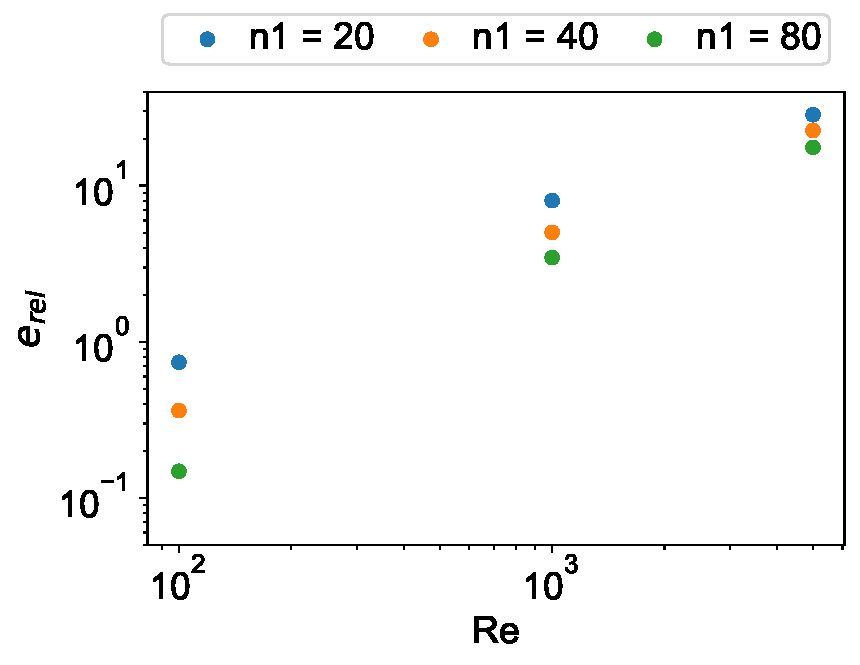
\includegraphics[width=\textwidth]{termino_adv_UP1.pdf}
      \caption{}
      \label{fig:termino_adv_UP1}
  \end{subfigure}
  \hfill
  \begin{subfigure}[b]{0.32\textwidth}
      \centering
      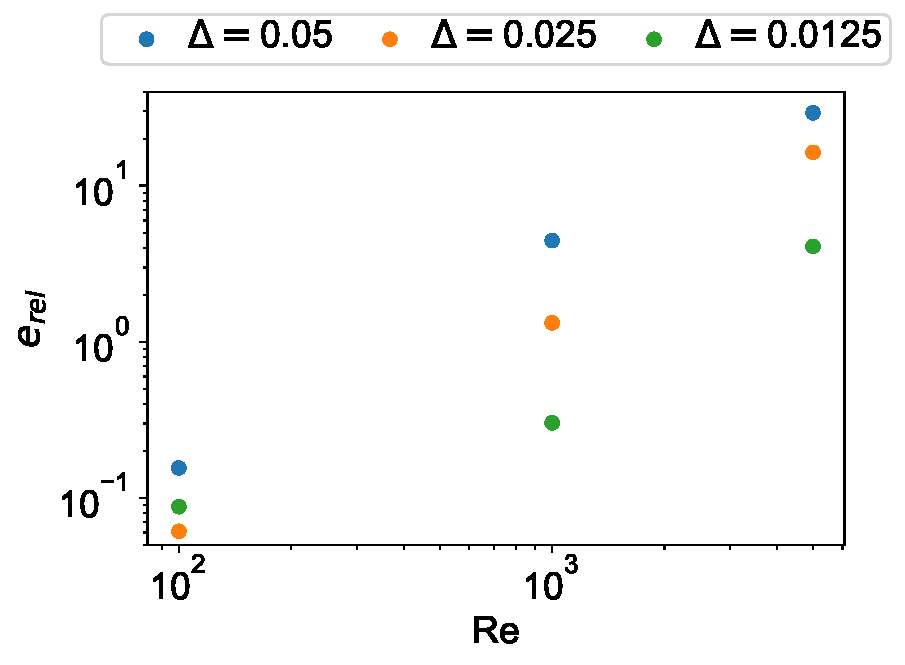
\includegraphics[width=\textwidth]{termino_adv_QUICK.pdf}
      \caption{}
      \label{fig:termino_adv_QUICK}
  \end{subfigure}
     \caption{Error relativo $e_{rel}$ para distintos número de Reynolds $Re$, tamaño de la discretización espacial $\Delta$ y método numérico para el término advectivo: (a) Diferencias centradas de orden 2, (b) Upwind de orden 1 y (c) método QUICK \textcolor{red}{ref}. En todos los casos se empló diferencias centradas de orden 2 para el término difusivo y Euler implícito para la evolución temporal.}
     \label{fig:termino_advectivo}
\end{figure}



\twocolumngrid



\begin{table}[]
  \begin{tabular}{l|lll|}
  \cline{2-4}
            & \multicolumn{3}{c|}{Re}                                     \\ \cline{2-4} 

            & \multicolumn{1}{c|}{100} & \multicolumn{1}{c|}{1000} &  \multicolumn{1}{c|}{5000} \\ \hline
  \multicolumn{1}{|l|}{DC2} & \multicolumn{1}{c|}{$0.08541$} & \multicolumn{1}{c|}{$0.17567$} & $0.69045$ \\ \hline
  \multicolumn{1}{|l|}{UP1} & \multicolumn{1}{c|}{$0.14813$} & \multicolumn{1}{c|}{$3.46833$} & $17.6402$ \\ \hline
  \multicolumn{1}{|l|}{QUICK} & \multicolumn{1}{c|}{$0.08778$} & \multicolumn{1}{c|}{$0.30266$} & $4.09139$ \\ \hline
  \end{tabular}
  \label{tabla:erel}
  \caption{Error relativo $e_{rel}$ para distintos número de Reynolds $Re$ y método numérico para el término advectivo: (a) Diferencias centradas de orden 2, (b) Upwind de orden 1 y (c) método QUICK \textcolor{red}{ref}. En todos los casos se empleó el tamaño de la discretización $\Delta = $ \textcolor{red}{valor}, diferencias centradas de orden 2 para el término difusivo y Euler implícito para la evolución temporal.}
\end{table}






\subsection{Orden de convergencia espacial de UP1}
Se calculó el orden de convergencia espacial del método UP1 para el término advectivo para $Re = 1$ y $1000$. Para ello se calculó el error en la determinación de $u(0.5, 0.2)$ y $v(0.2, 0.5)$ respecto a una solución precisa para distintos valores de $\Delta$. Se consideró como solución precisa a aquella con $n = 80$ y DC2 para el término advectivo, considerado como el método más preciso de los tres en base a los resultados presentados anteriormente. Se empleó el método Euler implícito para la evolución temporal y DC2 para el término de difusión.

\begin{itemize}
  \item Los resultados se grafican en la figura 
  \item En base al comportamiento lineal se realizó un ajuste de los datos, obteniendo como pendiente el orden de convergencia para $u$ y $v$ y $Re = 1$ y $1000$.
  \item En el caso de $Re = 1$ se obtuvo un orden de convergencia para $u$ de $2.5 \pm 0.3$ y para $v$ de $2.9 \pm 0.4$.
  \item Los órdenes de convergencia para cada variable son indistinguibles entre sí y mayores al orden teórico de UP1. Esto podría deberse a que a bajo número de Reynolds el término difusivo en las ecuaciones \ref{eq:momento_x} y \ref{eq:momento_y} cobra mayor importancia que el advectivo. Como el difusivo se discretizó con DC2 se esperaría un error del orden 2. Sin embargo, el orden de convergencia es aún mayor. No es claro a qué se debe este comportamiento pero podría estar relacionado a la mezcla de métodos espaciales y temporales utilzada y además, a que la solución de referencia no es la solución exacta sino una aproximación.
  \item En el caso de $Re = 1000$ se obtuvo un orden de convergencia para $u$ de $0.52 \pm 0.06$ y para $v$ de $0.52 \pm 0.05$. Ambos valores son indistinguibles entre sí y menores al orden teórico UP1. Análogamente al caso anterior, como aumentó el número de Reynolds, el término advectivo cobra mayor importancia y se esperaría un orden 1 de convergencia. Sin embargo, el orden es aún menor. No es claro a qué se debe este comportamiento pero podría deberse a las mismas razones discutidas para $Re = 1$.
\end{itemize}

\begin{figure}
  \centering
  \begin{subfigure}[b]{0.3\textwidth}
      \centering
      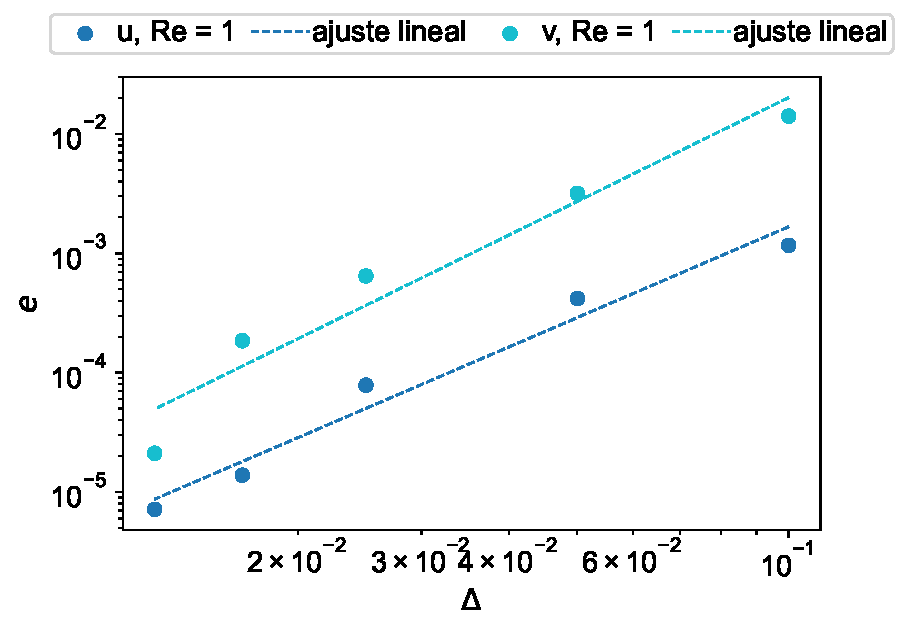
\includegraphics[width=\textwidth]{error_UP1_n1_vs_Re_1.pdf}
      \caption{}
      \label{fig:error_UP1_n1_vs_Re_1}
  \end{subfigure}
  \hfill
  \begin{subfigure}[b]{0.3\textwidth}
      \centering
      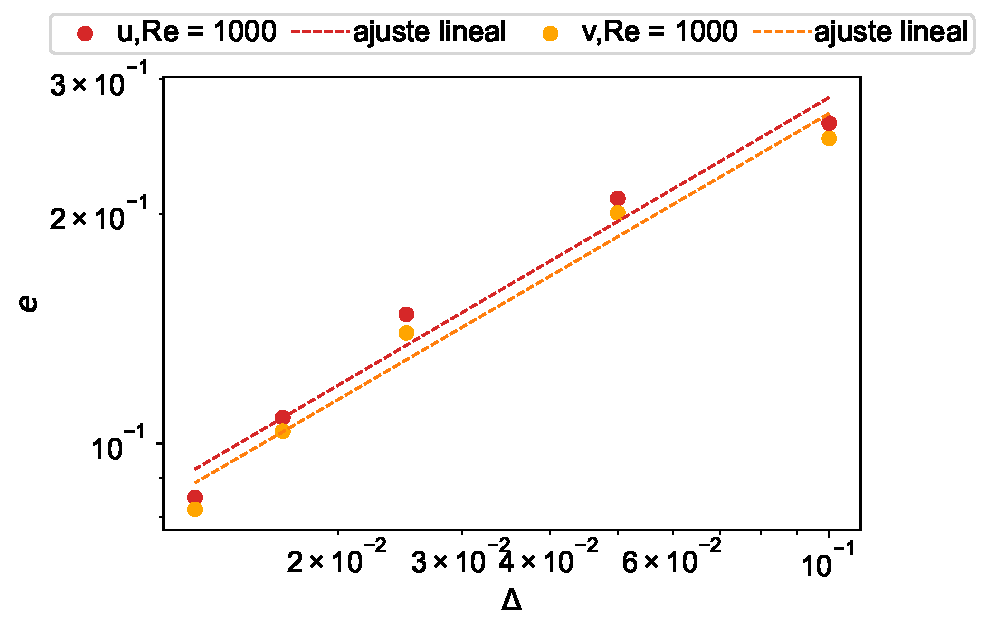
\includegraphics[width=\textwidth]{error_UP1_n1_vs_Re_1000.pdf}
      \caption{}
      \label{fig:error_UP1_n1_vs_Re_1000}
  \end{subfigure}
     \caption{Error local de $u$ y $v$ calculados con Upwind de orden 1 respecto a la solución con diferencias centradas de orden 2 para distintos valores de $\Delta$. Se analizaron los casos (a) $Re = 1$ y (b) $Re = 1000$. Se empleó el método Euler implícito para la evolución temporal y diferencias centradas de orden 2 para el término de difusión. Se ajustó en todos los casos una dependencia lineal $a \mathrm{log(\Delta)} + b$, donde $a$ indica el orden de convergencia. En el caso $Re = 1$ se obtuvo para $u$ una pendiente $a_{u}^1 = 2.5 \pm 0.3$ y para $v$, $a_{v}^1 = 2.9 \pm 0.4$. Mientras que en el caso $Re = 1000$ se obtuvo para $u$ una pendiente $a_u^1000 = 0.52 \pm 0.06$ y para $v$, $a_v^1000 ? 0.52 \pm 0.05$.
     }
     \label{fig:error_UP1_n1_vs_Re}
\end{figure}





\subsection{Esquema temporal con solución dependiente del tiempo}
\begin{itemize}
  \item Lo único que queda por estudiar es el efecto del método de evolución temporal en la solución numérica.
  \item Para esto se modificó la condición de contorno en la cara superior para que sea dependiente del tiempo como $U_0 = cos(t)$
  \item Se calculó la evolución temporal de $u(0.5,0.5)$ y $v(0.5,0.5)$ hasta $t = 10$ empleando Euler implícito y Crack-Nicholson. En cuanto a los parámetros de la simulación se empleó $n = 30$ y $Re = 1000$, DC2 para los término advectivo y difusivo, $\Delta t = 0.4$ y $l_{simpler} = 1$ y $3$. Los resultados se resumen en la figura

\end{itemize}


\textcolor{red}{Condición inicial?}
\textcolor{blue}{Evolución temporal con EI y CN.}








\section{Conclusión}

\bibliography{Chehade_final.bib}

\end{document}





